\documentclass[a4paper,10pt,twocolumn]{ltjsarticle}
\usepackage[haranoaji]{luatexja-preset}
\usepackage[top=18mm,bottom=20mm,left=17mm,right=17mm,columnsep=8mm]{geometry}
\usepackage{graphicx,booktabs,array,caption,enumitem,xcolor,tikz}
\usetikzlibrary{shapes.geometric}
\setlength{\parindent}{1\zw}
\renewcommand{\baselinestretch}{1.0}
\setlength{\parskip}{0pt}
\renewcommand{\thesection}{\arabic{section}.}
\renewcommand{\thesubsection}{\arabic{section}.\arabic{subsection}.}
\makeatletter
\renewcommand{\section}{\@startsection{section}{1}{\z@}{1.1\Cvs \@plus.4\Cdp \@minus.2\Cdp}{.5\Cvs \@plus.2\Cdp}{\normalfont\gtfamily\bfseries\large}}
\renewcommand{\subsection}{\@startsection{subsection}{2}{\z@}{.8\Cvs \@plus.3\Cdp \@minus.2\Cdp}{.3\Cvs \@plus.1\Cdp}{\normalfont\gtfamily\bfseries\normalsize}}
\makeatother
\captionsetup{font={small,sf},labelsep=space,justification=raggedright,singlelinecheck=false,skip=3pt}
\captionsetup[table]{position=top}
\setlist[itemize]{leftmargin=1.2\zw,itemsep=0pt,topsep=2pt,parsep=0pt}
\setlength{\textfloatsep}{8pt plus 2pt minus 2pt}
\setlength{\floatsep}{8pt plus 2pt minus 2pt}
\setlength{\intextsep}{8pt plus 2pt minus 2pt}
\pagestyle{plain}
\raggedbottom
\begin{document}
\twocolumn[{
\noindent\fbox{\gtfamily\small\ 生成AI論文\ }\par\medskip
\begin{center}
{\gtfamily\bfseries\LARGE 【高校情報科の担当教員】臨時免許状・免許外教科担任の自治体別人数（令和4年5月1日現在）$^{\dagger}$}\par\medskip
{\gtfamily\bfseries\large 臨時免許状・免許外教科担任の構成と自治体間の関連}\par\medskip
{\normalsize EduData調査研究グループ$^{*1}$・教育データサイエンス解析班$^{*2}$}\par
{\small オープン教育統計推進プロジェクト$^{*1}$・初等中等STEM教育データ基盤ユニット$^{*2}$}
\end{center}\smallskip
\noindent\begin{minipage}{\textwidth}\small 文部科学省の令和4年5月1日現在の資料から，高校の情報科を臨時免許状または免許外教科担任の許可で担当する教員の人数を，1人以上いる49自治体（全国65自治体のうち）について整理した．この49自治体の平均は，臨時免許状4.82人（中央値1.0人），免許外教科担任11.43人（中央値7.0人），計16.24人（中央値10.0人）であり，0人の16自治体を含まないため全自治体の平均ではない．計は長野県の76人が最も多く，栃木県の68人が続いた．臨時免許状と免許外教科担任の人数の相関は \textit{r}=−.01（\textit{n}=49）でほぼ0であったが，外れ値を除くと.16，両方が1人以上の25自治体に限ると.39となり符号が変わるため，関連の有無は決められない．また臨時免許状が0人の自治体が17，免許外教科担任が0人の自治体が7あり，分布が大きく偏っている．結果は自治体単位の集計値であり，個々の教員の因果や理由は示さない．\par\smallskip
\noindent{\gtfamily キーワード：}高校情報科，臨時免許状，免許外教科担任，自治体比較\end{minipage}\medskip
}]
\let\thefootnote\relax
\footnotetext{\footnotesize 2026年10月執筆\\ $^{\dagger}$Number of Teachers with Temporary Licenses or Non-Subject Licenses in High School Informatics by Municipality (as of May 1, 2022)†\\ $^{*1}$ Open Education Data Project, Tokyo, Japan\quad $^{*2}$ Educational Data Science Unit, Tokyo, Japan}
\section{はじめに}
\subsection{研究の背景}
高校の情報科の授業は，学習指導要領（平成30年告示）の解説（文部科学省，2019）が示す内容を，担当教員が実現することで成り立つ．令和7年度の大学入学共通テストについても問題作成方針が公表されており（大学入試センター，2023），高校の教科指導の体制は入学者選抜とも無関係ではない．

教員の力量をめぐっては，Shulman (1986)が教える内容と教え方にまたがる教師の知識の成長を論じ，Mishra and Koehler (2006)はそれを技術の知識まで広げた TPACK の枠組みを示した．Wing (2006)は計算論的思考を論じており，情報科の内容と関わる．ただし免許状の有無は，これらの知識の水準を直接測る指標ではない．資格の不十分な教員の問題は，Ingersoll (1999)が米国の中等学校について論じており，Hubwieser et al. (2015)は世界各地のK-12のコンピュータ科学教育の状況を整理している．

日本では，文部科学省 (2022)が高校の情報科の担当教員の配置状況を公表している．本研究はこの資料を用い，臨時免許状と免許外教科担任の人数が自治体によってどう異なるか，両者の人数に関連があるかを記述する．
\subsection{リサーチクエスチョン}
本研究の目的は，高校の情報科を臨時免許状または免許外教科担任の許可で担当する教員の人数を自治体別に整理し，その構成と自治体間の関連を記述することである．
\begin{itemize}
\item RQ1：臨時免許状・免許外教科担任の計が多いのはどの自治体か．臨時免許状と免許外教科担任の構成は，自治体でどう違うか．
\item RQ2：臨時免許状の人数が多い自治体は免許外教科担任の人数が少ないという関係があるか（両者の人数の関連）．
\end{itemize}
\section{調査対象および分析方法}
文部科学省 (2022)の資料から，臨時免許状・免許外教科担任が1人以上いる49自治体（都道府県と政令指定都市，全国65自治体のうち）の人数を用いた．0人の16自治体は表に載っていないため，対象に入っていない．分析単位は自治体で，各自治体を同じ重みで扱った．したがって平均や中央値は自治体の値の平均であり，教員数で重みづけした値でも全65自治体の値でもない．人数は実数で，高校数や教員数で割った値ではない．

相関はピアソンの \textit{r}，95\%信頼区間，スピアマンの \textit{ρ}，\textit{p}，JZSベイズファクター \textit{BF}\textsubscript{10}（尺度1）で示した．6つの指標から計算でつながる組を除いた12組を探索し，多重比較の基準はボンフェローニ法の.05÷12（約.004）とした．RQ2に関わる1組のみを結果として報告する．結果が特定の自治体に依存しないかを確かめるため，上位2自治体（長野県，栃木県）を除いた場合，計の上位5自治体を除いた場合，臨時免許状または免許外教科担任の人数が四分位範囲の1.5倍の基準を超える外れ値の自治体（8自治体）を除いた場合，計が2人以下の9自治体を除いた場合，1自治体ずつ除いた場合の \textit{r} を元データから求めた．
\begin{table*}[!t]
\caption{主要指標の基本記述統計量}
\centering\small
\begin{tabular}{>{\raggedright\arraybackslash}p{9.2cm}rrrrrr}
\toprule
指標 & \textit{K} & 平均 & \textit{SD} & 中央値 & 最小 & 最大 \\
\midrule
臨時免許状 & 49 & 4.8 & 9.1 & 1.0 & 0.0 & 45.0 \\
免許外教科担任 & 49 & 11.4 & 14.0 & 7.0 & 0.0 & 76.0 \\
臨時免許状・免許外教科担任の計 & 49 & 16.2 & 16.6 & 10.0 & 1.0 & 76.0 \\
計の令和2年調査からの増減 & 49 & -8.9 & 18.8 & -4.0 & -93.0 & 8.0 \\
令和5年4月見込み（改善計画の履行後） & 49 & 1.6 & 5.2 & 0.0 & 0.0 & 29.0 \\
情報免許状保有で情報科を担当していない者 & 49 & 101.4 & 69.4 & 81.0 & 0.0 & 347.0 \\
\bottomrule
\end{tabular}
\par\smallskip{\footnotesize 注）単位は人，\textit{K}は観測数（国・地域・区分）．}
\end{table*}
\begin{table*}[!t]
\caption{主要指標間のピアソンの相関係数と，ベイズファクター}
\centering\small
\begin{tabular}{>{\raggedright\arraybackslash}p{6.4cm}>{\raggedright\arraybackslash}p{6.4cm}rrr}
\toprule
指標 \textit{X} & 指標 \textit{Y} & \textit{r} & \textit{p} & \textit{BF}\textsubscript{10} \\
\midrule
臨時免許状 & 免許外教科担任 & −.01 & = .923 & 0.11 \\
臨時免許状 & 計の令和2年調査からの増減 & −.16 & = .260 & 0.21 \\
臨時免許状 & 令和5年4月見込み（改善計画の履行後） & .15 & = .299 & 0.19 \\
臨時免許状 & 情報免許状保有で情報科を担当していない者 & −.04 & = .786 & 0.12 \\
免許外教科担任 & 計の令和2年調査からの増減 & −.49 & < .001 & 57.87 \\
\bottomrule
\end{tabular}
\par\smallskip{\footnotesize 注）\textit{BF}\textsubscript{10}はJZSベイズファクター（3を超えれば関連を支持，1/3を下回れば関連がないことを支持）．全ペアの探索の一部を載せた．}
\end{table*}
\section{結果}
49自治体における臨時免許状・免許外教科担任の計は，平均16.24人（中央値10.0人）であり，平均より多い自治体は19であった．全国の合計は臨時免許状236人，免許外教科担任560人，計796人で，情報科担当教員4756人のうちの人数である．

RQ1について，計が多い自治体の上位5つは，長野県（76人），栃木県（68人），福島県（45人），茨城県（40人），北海道（39人）であった．計が最も少ない1人の自治体は7つあり（佐賀県，山口県，大阪府，京都府，札幌市，京都市，福岡市），同順位である．これらは人数であって割合ではないため，自治体の規模の違いも含む．内訳では，臨時免許状は栃木県（45人），鹿児島県（35人），茨城県（30人）で多く，免許外教科担任は長野県（76人），福島県（45人），北海道（39人）で多かった．臨時免許状が0人の自治体は17，免許外教科担任が0人の自治体は7（鹿児島県，福井県，広島市，京都府，札幌市，京都市，福岡市），両方が1人以上の自治体は25であった．

RQ2について，臨時免許状と免許外教科担任の相関は \textit{r}=−.01（95\%CI [−0.29, 0.27]，\textit{ρ}=−.05，\textit{n}=49，\textit{p}=.923，\textit{BF}\textsubscript{10}=0.11）であった．\textit{BF}\textsubscript{10}は1/3未満だが，分布が大きく偏っているため目安にとどめる．上位2自治体を除くと \textit{r}=−.09（\textit{n}=47），計の上位5自治体を除くと \textit{r}=−.03（\textit{n}=44），計が2人以下の自治体を除くと \textit{r}=−.10（\textit{n}=40），1自治体ずつ除くと \textit{r} は-.12から.05の範囲で，いずれも0に近かった．一方，外れ値の8自治体を除くと \textit{r}=.16（\textit{n}=41），両方が1人以上の25自治体に限ると \textit{r}=.39（\textit{ρ}=.37，\textit{p}=.056）となり，符号は除き方で変わった．対照として，臨時免許状と，情報免許状を持ちながら情報科を担当していない者の人数との相関は \textit{r}=−.04（\textit{BF}\textsubscript{10}=0.12），免許外教科担任との相関は \textit{r}=.15（\textit{BF}\textsubscript{10}=0.19）で，いずれもRQ2の相関と同様に0に近いか弱かった（これらは参考値で，対照としての意味づけはしない）．探索した12組のうち，基準を満たしたのは4組（\textit{p}<.001）で，いずれもRQ2に関わらないため扱わない．計が0人の16自治体を加えた65自治体では，相関は\textit{r}=.08であった．また資料には令和2年調査からの計の増減があり，49自治体の増減の和は-434人（減少）であった．
\begin{figure}[t]\centering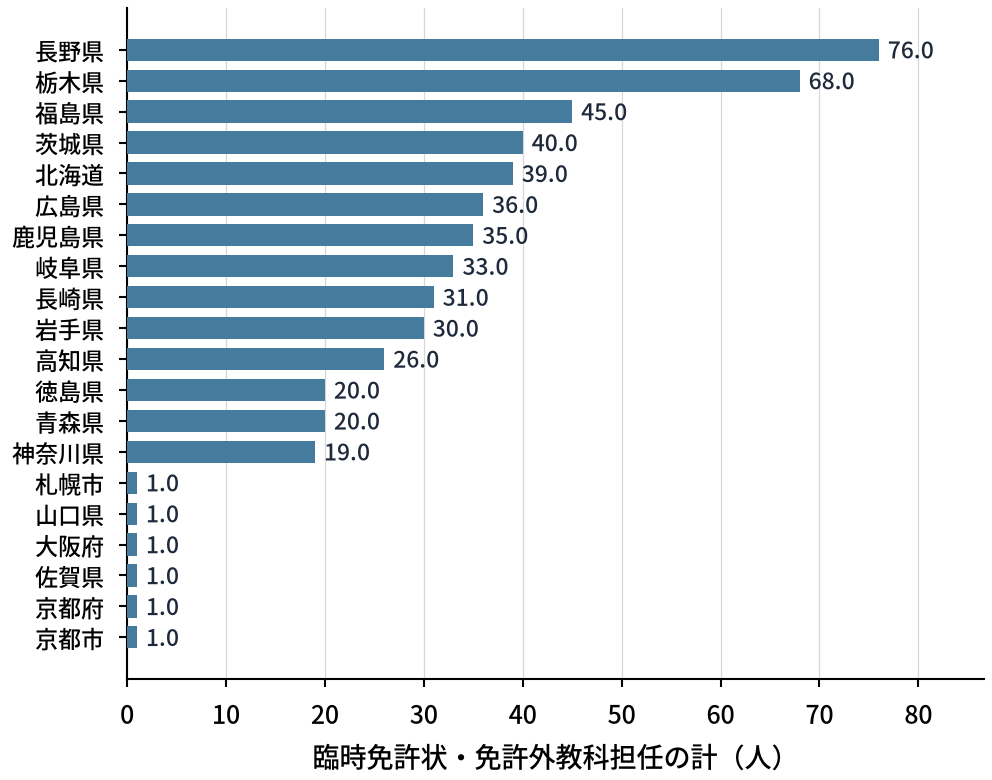
\includegraphics[width=\columnwidth]{chart_japan_high_school_informatics.png}\caption{臨時免許状・免許外教科担任の計の値の比較（上位・下位と日本を抜粋）．赤が日本}\end{figure}
\begin{figure}[t]\centering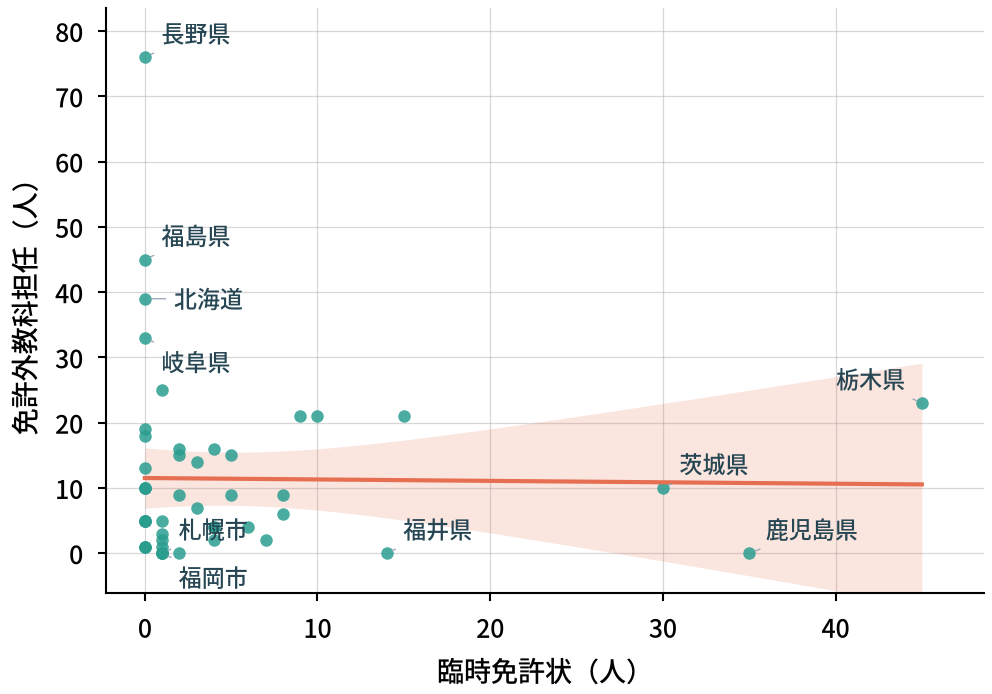
\includegraphics[width=\columnwidth]{chart_secondary_japan_high_school_informatics.png}\caption{臨時免許状と免許外教科担任の関連（回帰直線と，その平均の95\%信頼区間の帯，n=49）}\end{figure}
\section{考察}
RQ1では，計は自治体によって大きく異なり，上位の自治体では数十人であった．一方で計が1人の自治体も7あり，順位だけでなく同順位の多さにも注意が必要である．内訳では，臨時免許状が多い自治体（栃木県，鹿児島県）と免許外教科担任が多い自治体（長野県，福島県）があり，どちらか一方だけの自治体と両方を使う自治体に分かれていた．

RQ2では，全49自治体で臨時免許状と免許外教科担任の人数に直線的な関連は見られなかった．ただし0人の自治体が多く分布が偏っているため，外れ値を除いた場合や両方が1人以上の自治体に限った場合には符号が変わった．確かな結論は出せず，除き方に依存しない関連があるとは言えない．自治体ごとの違いの理由として，採用や配置の方針，免許状の取得支援の違いなどが考えられるが，仮説にとどまり，本研究のデータでは検証できない．Ingersoll (1999)が論じた資格の問題を日本の免許外教科担任に当てはめる場合も，免許状の有無は授業の質を直接示さない点に注意が要る．

限界は，(1)自治体単位の集計値のみで，個々の教員の因果を特定できないこと（生態学的誤謬），(2)臨時免許状・免許外教科担任が1人以上いる49自治体のみで，全65自治体ではないこと，(3)調査の回答方法は資料から確認できず，人数は令和4年5月1日の1時点で分析しており，令和2年調査からの変化を自治体ごとには分析していないこと，(4)高校数・教員数で割っておらず，授業の質や生徒の学力，採用状況などの交絡を統制していないこと，である．Shulman (1986)やMishra and Koehler (2006)が論じた教師の知識は，このデータでは測れていない．教育現場での指導体制の改善の効果は，確かめられていない．
\section*{参考文献}
\begingroup\scriptsize\raggedright\interlinepenalty=10000 
\begin{list}{}{\setlength{\leftmargin}{1.5\zw}\setlength{\itemindent}{-1.5\zw}\setlength{\labelwidth}{0pt}\setlength{\labelsep}{0pt}\setlength{\itemsep}{1pt}\setlength{\parsep}{0pt}\setlength{\topsep}{0pt}\setlength{\listparindent}{0pt}}
\item HUBWIESER, P., GIANNAKOS, M. N., BERGES, M., BRINDA, T., DIETHELM, I., MAGENHEIM, J., PAL, Y., JACKOVA, J. and JASUTE, E. (2015) A global snapshot of computer science education in K-12 schools. Proceedings of the 2015 ITiCSE on Working Group Reports, 65-83.
\item INGERSOLL, R. M. (1999) The problem of underqualified teachers in American secondary schools. Educational Researcher, \textbf{28} (2) ：26-37.
\item MISHRA, P. and KOEHLER, M. J. (2006) Technological pedagogical content knowledge: A framework for teacher knowledge. Teachers College Record, \textbf{108} (6) ：1017-1054.
\item 文部科学省 (2019) 高等学校学習指導要領（平成30年告示）解説 情報編. 開隆堂出版.
\item 文部科学省 (2022) 高等学校情報科担当教員の配置状況及び指導体制の充実に向けて（令和4年11月）. 文部科学省初等中等教育局学校デジタル化PT.
\item 大学入試センター (2023) 令和7年度大学入学者選抜に係る大学入学共通テスト問題作成方針. 独立行政法人大学入試センター.
\item SHULMAN, L. S. (1986) Those who understand: Knowledge growth in teaching. Educational Researcher, \textbf{15} (2) ：4-14.
\item WING, J. M. (2006) Computational thinking. Communications of the ACM, \textbf{49} (3) ：33-35.
\end{list}\endgroup
\section*{Summary}
{\footnotesize\setlength{\parindent}{0pt}Using data from the Ministry of Education, Culture, Sports, Science and Technology (2022), we organized the number of teachers who teach high school informatics with temporary licenses or non-subject licenses across the 49 of 65 municipalities that had at least one such teacher. The total averaged 16.24 (median 10.0) per municipality. The correlation between the two numbers was r = −.01 (95\% CI [−0.29, 0.27], n = 49, p = .923, BF10 = 0.11), supporting no association, but the sign changed when outliers were removed or when the sample was limited to municipalities with both types. These results are descriptions of municipality-level aggregates and do not imply causation for individual teachers.\par\smallskip KEYWORDS: High School Informatics, Temporary License, Non-Subject License, Municipality Comparison\par}
\medskip\noindent\fbox{\parbox{\dimexpr\columnwidth-2\fboxsep-2\fboxrule}{\footnotesize\gtfamily 【付記：生成AIによる自動執筆に関する開示】\\ 本論文は学生への教育目的で作成している．使用しているデータは公的オープンデータである．統計の算出はPythonで行い，文章は生成AI（Anthropic Claude等）を活用して作成した．記載した統計数値は元データに準拠しているが，教育学的な考察や提言の妥当性は，指導現場の実情に応じて，批判的に吟味してほしい．}}
\end{document}
